%!TEX root = ../thesis.tex

% TODO:
% 1. Improve quality.
% 2. Make sure we have a reference for everything. (e.g. add einstein paper)
% 3. Finish the "organized" part at the end.
% 4. Improve quality of Figure 1.
% 5. Maybe add that this is the basic for a project where new physics should
%    be found like e.g. NS eq. of state blabla.

\section{Introduction}
% Introduction to the general topic of GW
In 1916, Einstein predicted the existence of gravitational waves. With the first
detection of a gravitational wave\cite{PhysRevLett.116.061102}, emitted by two 
merging black holes, on September 14, 2015 his prediction was profen correct.
This detection marked the beginning
of the GW astronomy era. Up until then, it was also the last missing
 extrasolar messenger needed for full-scale multi-messenger physics.
\cite{Branchesi_2016} 

% Multi-Messenger physics: Importance of latency
Because multi-messenger physics utilizies different messengers to observe the 
same transient, it is of paramount interested to minimize the latency between 
the transient's actual occurence and its reported detection.

% Descibe the current situation: We have several detectors. The measurement is
% noisy.
When analyzing the \textit{strain} $s(t)$ measured by the detector, the
fundamental assumption is that it is made up by the GW \textit{signal} $h(t)$
and \textit{noise} $n(t)$ whereas

\begin{equation}
  s(t) = n(t) + h(t)
\end{equation}

Analyzing $s(t)$ about the possibile occurence of $h(t)$ is currently done by
using an approach called matched filtering. Matched filtering works by 
convoluting precalculated
models of expected signals, so called templates, with the measured data.
Because the parameters of the expected signals are not known in advance, the
template bank spans a large astronomical parameter space. This leads to
matched filtering approaches being very computationally expensive which leads
to a high latency between the occurence of the GW signal and the reported
detection. It is therefor of interest to find methods which are less
computationally expensive and thus provide a low-latency detection algorithm.


In \autoref{fig:1_data_processing}, taken from \cite{2020CQGra..37e5002A},
we can see a simplified schematic summarizing the main steps in LIGO-Virgo data
processing.  It starts with the measurement done by the detector. The
measurement undergoes a quality control to make sure the measurement is actually
useful. Once a sufficient quality has been established, the data is being
searched for GW signals and in case a signal is found (called an event),
the mergers parameters are being estimated. Each event gets a statistical
significance assigned, which is usually given by the false-alarm rate (FAR)
of the search at a ranking statistic threshold associated with the candidate 
event. The FAR is basically telling us how many false positives occured over
the duration of the analyzed data. Current low-latency searches do not distribute
any event candidates with a FAR greated than 1 per month.



% OKAY

% I now want to establish the FAP vs. FAR issue.

%Because a detector has to be upgraded and maintained it can't run all the time.
%This together with the quality control leads to the data stream being split up
%into segments. Each segment is several days to several weeks long. When
%searching for signals or trying to estimate parameters, we can't directly pass
%a whole segment. This is because a segment usually contains too much data at
%once but also because different segments have different durations. This issue is
%solved by using a sliding window of fixed duration, e.g. 1 second, and a stride
%of fixed
%duration, e.g. 0.1 second. The window is then being moved through the segment
%using the stride. E.g. a segment of 10 seconds would results in 90 one second
%mini-segments. Each such mini-segment is then passed to the needed algorithm.
%The algorithm gives a result about this 1 second of data. E.g. it might tell us
%that this 1 second of data contains a (a art of) a signal. This is called a
%trigger.
%
%The above approach of using a sliding window to feed the data to an algorithm
%leads to several sliding window giving a trigger for the same GW
%signal. Because we only want one positive alarm per GW signal, we cluster
%together close triggers.


% Describe what previous work did.

% Say what's wrong with previous work

% Make a conclusion: FAP vs FAR


Pioneering works by XX and XX showed that convolutional neural network can
distinguish between a sample containing only pure noise and noise injected
with a signal from BBH. Those works both used a similar setting. They used either
simulated gaussian or real LIGO noise and injected simulated signals into it.
Each such sample was 1s long. They used those samples to train their CNN but
also as their test set. To evaluate their network, they used the commonly used
true ositive rate and the false positive rate and computed a ROC curve using
false alarm probability. As [29] showed, this is an issue because the actual
data of a detector is continuous stream of data. False alarm probability is a
way better way to compare a deep learning algorithm to a matched filter
algorithm.

The networks tested in these works were able to distinguish
data containing a GW signal from pure noise with a false alarm probability (FAP)
of $10^{-3}$ i.e. the networks classified about 1 in 1000 pure noise samples
falsly as containing a signal.

In [29] it was shown that this approach (FAPs) does not directly translate to
false alarm rates (FARs) on continous data streams. The appropriate question to
asl is: How many false signals does the network identify per time interval of
continous data, as opposed to how many uncorrelated data chunks are falsely
identified as containing a signal. Furthermore, comparing deep learning to
matched filtering is hard because the later works on way lower FARs.


In this thesis,
we will explore a similar deep learning (DL) approach to search for simulated GW
signals in simulated Gaussian noise. While training a neural network (NN) is also
rather computationally expensive, the evaulation of a trained NN can be done in
a fraction of a second. Furthermore future detections can easily be incorporated
leading to an improved neural network.

TODO: Because this work might become the fundation for a bigger project and
because it was approached in a very open way, the code is rather general and
easily extendable to a more general case.

TODO: Add paragraph about basic functionality of a DL approach (epoch etc.)

TODO: Add paragraph about "this thesis was very open, thus I started with a
broad approach, thus the thesis supports quit a bit of shit it doesn't need"

This thesis is organized as follows. In Section 2 we first establish the data
used for our DL approach, so we know what we actually work with. In section 3 
we will describe the actual DL approach.
In section 4, we present the results. In section 5 we discuss possibilities for 
future work.

\begin{figure}
  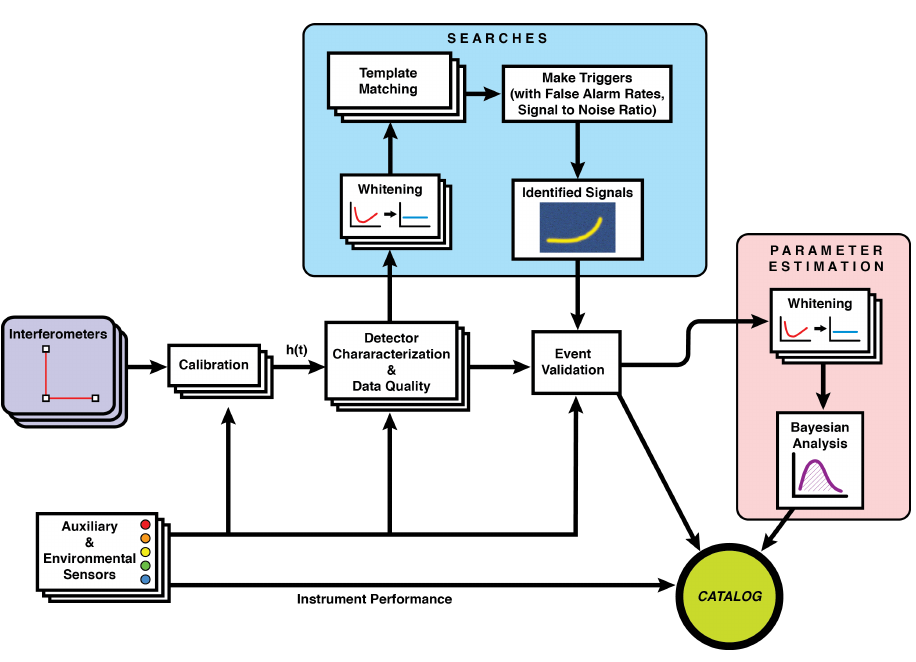
\includegraphics[width=\textwidth]{img/1_introduction/data_processing.png}
  \caption{asd}
  \label{fig:1_data_processing}
  \centering
\end{figure}



